%%%%%%%%%%%%%%%%%%%%%%%%%%%%%%%%%%%%%%%%%
% Wenneker Assignment
% LaTeX Template
% Version 2.0 (12/1/2019)
%
% This template originates from:
% http://www.LaTeXTemplates.com
%
% Authors:
% Vel (vel@LaTeXTemplates.com)
% Frits Wenneker
%
% License:
% CC BY-NC-SA 3.0 (http://creativecommons.org/licenses/by-nc-sa/3.0/)
% 
%%%%%%%%%%%%%%%%%%%%%%%%%%%%%%%%%%%%%%%%%

%----------------------------------------------------------------------------------------
%	PACKAGES AND OTHER DOCUMENT CONFIGURATIONS
%----------------------------------------------------------------------------------------

\documentclass[11pt]{article} % Font size

%%%%%%%%%%%%%%%%%%%%%%%%%%%%%%%%%%%%%%%%%
% Wenneker Assignment
% Structure Specification File
% Version 2.0 (12/1/2019)
%
% This template originates from:
% http://www.LaTeXTemplates.com
%
% Authors:
% Vel (vel@LaTeXTemplates.com)
% Frits Wenneker
%
% License:
% CC BY-NC-SA 3.0 (http://creativecommons.org/licenses/by-nc-sa/3.0/)
% 
%%%%%%%%%%%%%%%%%%%%%%%%%%%%%%%%%%%%%%%%%

%----------------------------------------------------------------------------------------
%	PACKAGES AND OTHER DOCUMENT CONFIGURATIONS
%----------------------------------------------------------------------------------------

\usepackage{amsmath, amsfonts, amsthm} % Math packages

\usepackage{float}

\usepackage{color}

\usepackage{listings} % Code listings, with syntax highlighting

\usepackage[english]{babel} % English language hyphenation

\usepackage{graphicx} % Required for inserting images
\graphicspath{{Figures/}{./}} % Specifies where to look for included images (trailing slash required)

\usepackage{booktabs} % Required for better horizontal rules in tables

\numberwithin{equation}{section} % Number equations within sections (i.e. 1.1, 1.2, 2.1, 2.2 instead of 1, 2, 3, 4)
\numberwithin{figure}{section} % Number figures within sections (i.e. 1.1, 1.2, 2.1, 2.2 instead of 1, 2, 3, 4)
\numberwithin{table}{section} % Number tables within sections (i.e. 1.1, 1.2, 2.1, 2.2 instead of 1, 2, 3, 4)

\setlength\parindent{0pt} % Removes all indentation from paragraphs

\usepackage{enumitem} % Required for list customisation
\setlist{noitemsep} % No spacing between list items

%----------------------------------------------------------------------------------------
%	DOCUMENT MARGINS
%----------------------------------------------------------------------------------------

\usepackage{geometry} % Required for adjusting page dimensions and margins

\geometry{
	paper=a4paper, % Paper size, change to letterpaper for US letter size
	top=2.5cm, % Top margin
	bottom=3cm, % Bottom margin
	left=3cm, % Left margin
	right=3cm, % Right margin
	headheight=0.75cm, % Header height
	footskip=1.5cm, % Space from the bottom margin to the baseline of the footer
	headsep=0.75cm, % Space from the top margin to the baseline of the header
	%showframe, % Uncomment to show how the type block is set on the page
}

%----------------------------------------------------------------------------------------
%	FONTS
%----------------------------------------------------------------------------------------

\usepackage[utf8]{inputenc} % Required for inputting international characters
\usepackage[T1]{fontenc} % Use 8-bit encoding

\usepackage{fourier} % Use the Adobe Utopia font for the document

%----------------------------------------------------------------------------------------
%	SECTION TITLES
%----------------------------------------------------------------------------------------

\usepackage{sectsty} % Allows customising section commands

\sectionfont{\vspace{6pt}\centering\normalfont\scshape} % \section{} styling
\subsectionfont{\normalfont\bfseries} % \subsection{} styling
\subsubsectionfont{\normalfont\itshape} % \subsubsection{} styling
\paragraphfont{\normalfont\scshape} % \paragraph{} styling

%----------------------------------------------------------------------------------------
%	HEADERS AND FOOTERS
%----------------------------------------------------------------------------------------

\usepackage{scrlayer-scrpage} % Required for customising headers and footers

\ohead*{} % Right header
\ihead*{} % Left header
\chead*{} % Centre header

\ofoot*{} % Right footer
\ifoot*{} % Left footer
\cfoot*{\pagemark} % Centre footer
 % Include the file specifying the document structure and custom commands

\title{	
	\normalfont\normalsize
	
\includegraphics[width=0.5\columnwidth]{logo-black}
	%\textsc{Molo17 S.r.l.}\\ % Your university, school and/or department name(s)
	\vspace{25pt} % Whitespace
	\rule{\linewidth}{0.5pt}\\ % Thin top horizontal rule
	\vspace{20pt} % Whitespace
	{\huge Event-Driven cloud architectures, CQRS and Event Sourcing}\\ % The assignment title
	\vspace{12pt} % Whitespace
	\rule{\linewidth}{2pt}\\ % Thick bottom horizontal rule
	\vspace{12pt} % Whitespace
}

\author{\LARGE Lorenzo Busin} % Your name

\date{\normalsize August, 2019} % Today's date (\today) or a custom date

\begin{document}

\maketitle % Print the title

%\section{Image Interpretation}

%\begin{figure}[h] % [h] forces the figure to be output where it is defined in the code (it suppresses floating)
	%\centering
	%\includegraphics[width=0.5\columnwidth]{swallow.jpg} % Example image
	%\caption{European swallow.}
%\end{figure}
\tableofcontents
\newpage

\section{Event-Driven architectures}  

\subsection{What is an Event-Driven architecture?}
Event-Driven architecture is a popular distributed asynchronous architecture pattern used to produce highly scalable and adaptable applications. It is made of highly decoupled and single-purpose event processing components that receive and process events. 

\subsection{What is an event?}
An event is an action recognized and handled by the software, often asynchronously. Events can be generated or triggered by the system, the user or in other ways. The software can also trigger its own set of events to forward information to other services or communicate with them. An application that changes its behavior in response to events is called "Event-Driven".\\
The main difference between commands and events is that the firsts say to the system \emph"This is what you have to do" while the seconds just say \emph{"This is happened"} and then is up to the handler to decide what to do.

\subsection{What is Event-Driven programming?}
Event-Driven programming is a programming paradigm where the flow of the program is determined by events such as user actions, sensor outputs or messages from other programs. This paradigm is mostly used in graphical user interfaces and other applications such as JavaScript web apps that are centered on performing actions in response to inputs. \\
In an Event-Driven application there is a main loop that listens for events and then triggers a callback function when one of those is detected. The events' listener is a common thing among applications, for this reason many programming frameworks take care of their implementation and expect the user to provide only the code for the event handlers.

\subsection{Events communication}
Events just communicate that something happened, so thanks to them you let a system know that something has happened. When an event occurs it will activate its handler which implements the execution logic. The result of the event's execution can turn into changes in the model-view or can trigger other handlers by forwarding it. \\
The \emph{observer} pattern is a flawless example of how events communicate with each other. 
\begin{figure} [H]
	\centering
	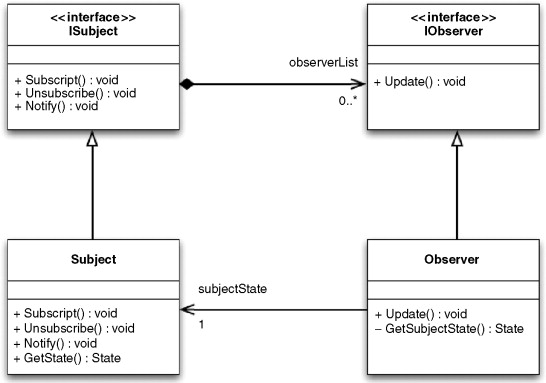
\includegraphics[scale=0.8]{observer}
\end{figure}
A subject maintains a list of its  observers and notifies them automatically of any state changes, usually by calling one of their methods.
This design pattern is mainly used to implement distributed event handling systems and is also a key part in MVC pattern.\\ 

According to \emph{Martin Fowler}, there are two ways of communicating between events: \textbf{Event notification} and \textbf{Event-Carried State Transfer}.

\subsubsection{Event notification}
To understand how Event notification works we can think of when our smartphone notifies us that a new message has arrived without adding any information. This happens when a system sends event messages to notify other systems of a change in its domain. The receiver knows something has changed but then issues a request back to the sender to decide what to do next, sending a request message and receiving a response for every event that happened. \\
The key element of Event notification is that the source system doesn't really care much about the response. So if the event's body does not need, Event notification is an excellent solution as it guarantees decoupling and high performance.

\subsubsection{Event-Carried State Transfer}
To understand how Event-Carried State Transfer works we can think of when our smartphone notifies us that a new message has arrived but in this case it shows other information like the sender's name and the message content. When something changes, the generated event contains the details of what has been changed. In this way the receiver does not need to ask the sender what has been changed.\\
A down-side of this model is that the messages that are sent contain more data but this fact reduces latency, because it is not necessary to query the source for further details. It does involve more complexity on the receiver since it has to sort out maintaining all the state, when it's usually easier just to call the sender to obtain more information.\\
So if the receiver needs to know extra data with the event object, Event-Carried State Transfer is an excellent solution as it guarantees better performance and lower demands on the supplier but more expensive communications.


\subsection{Event-Driven architecture's topologies}
Event-Driven architecture consists of two main topologies: \textbf{mediator} and \textbf{broker}. The mediator one is commonly used when you need to orchestrate multiple steps within an event through a central mediator, while the broker topology is used when you want to chain events together without the use of a central mediator.

\subsubsection{Mediator topology}
The mediator topology is useful for events that have multiple steps and require some level of orchestration to process the event. For example, a single event may consist of multiple steps that would require a certain level of orchestration to determine their order of execution. \\
There are four main types of architecture components within the mediator topology: event \emph{queues}, an event \emph{mediator}, event \emph{channels} and event \emph{processors}. \\
The event flow starts with a client sending an event to an event queue, which is used to transport the event to the mediator. It receives the initial event and orchestrates that event by sending additional events to event channels. Then, the event processors listen on the channels, receive the event and execute specific business logic.

\begin{figure} [H]
	\centering
	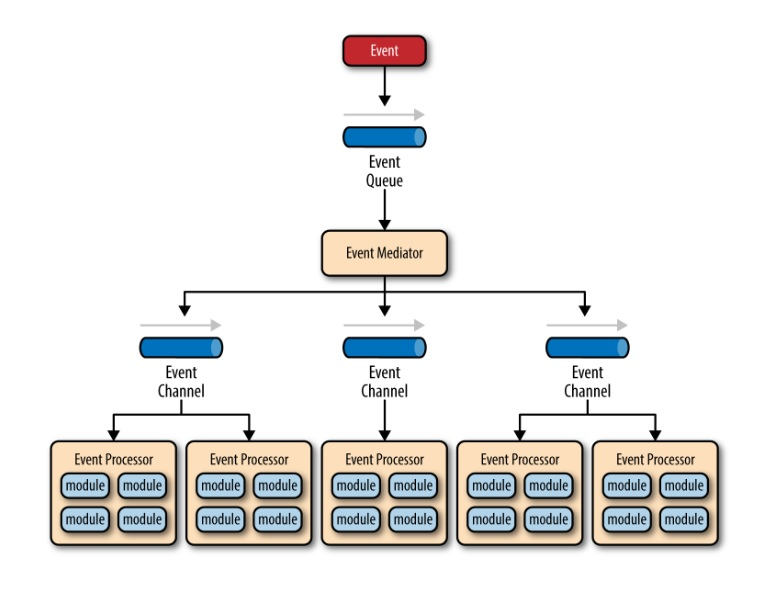
\includegraphics[scale=0.8]{mediator}
\end{figure}
There are two types of events within this pattern: an initial event and a processing event. The initial event is the original event received by the mediator, whereas the processing events are the ones that are generated by the mediator and received by the event-processing components.\\
The event-mediator component is responsible for orchestrating the steps contained within the initial event. For each step, the mediator sends out a specific processing event to an event channel, which is received and executed by the event processor. It is important to note that the event-mediator doesn't perform any business logic.\\
The event channels can be either message queues or message topics; the seconds are widely used with the mediator topology because the events can be processed by multiple event processors.\\
The event-processors contain the business logic necessary to process events. They are self-contained, independent and highly decoupled that perform a specific task in the application or system. It is important to keep in mind that each event-processor component should perform a single business task and not rely on others to complete it.
\subsubsection{Broker topology}
The broker topology is different from the mediator topology because there is no central event mediator. The message flow is distributed across the event processor components in a chain through a lightweight message broker. This topology is useful when you have a simple event processing flow.

\begin{figure} [H]
	\centering
	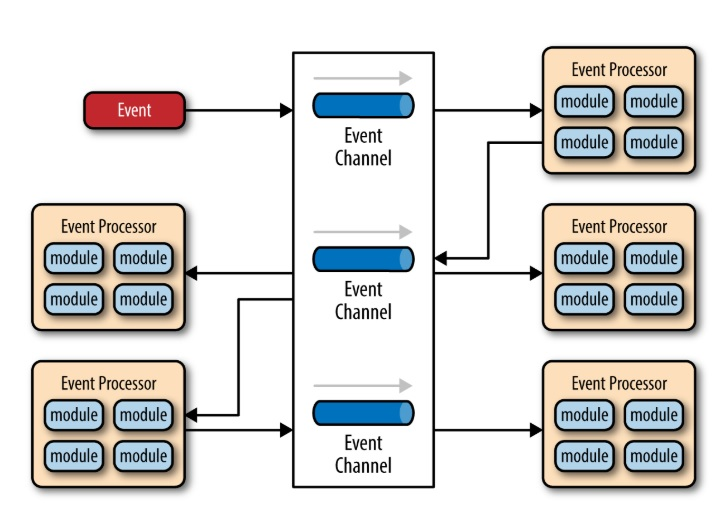
\includegraphics[scale=0.8]{broker}
\end{figure}

As you can see from the diagram, there is no central event-mediator controlling and orchestrating the initial event. Each event-processor component is responsible for processing events and publishing new events related to the action just performed. When an event processor receives an initial event, it performs its business logic and then publishes a new event to the broker, which would then be picked up by a different event processor. 

\subsubsection{Hybrid topology}
The use of one or more mediators may cause a tightly coupled system with strong dependencies. Can be hard instead to implement and to handle a broker topology because of the complex event flow.\\
In complex and intricate systems the best choice is tho adopt an hybrid topology mixing the pros of both to efficiently handle the application workflow. 


\subsection{Pattern analysis}
\begin{figure} [H]
	\centering
	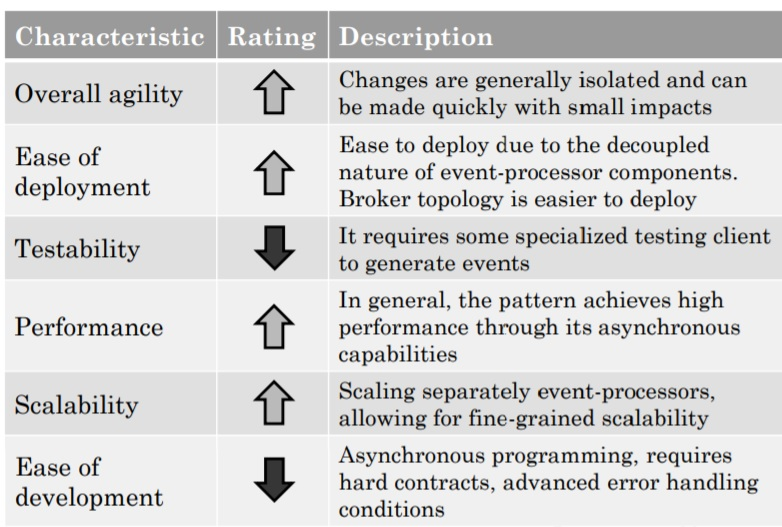
\includegraphics[scale=0.65]{analysis}
\end{figure}
\definecolor{darkgreen}{rgb}{0.0, 0.5, 0.0}
 \textbf{Overall agility}(\color{darkgreen}High\color{black}): is the ability to respond quickly to a constantly changing environment. Since event-processor components are single-purpose and completely decoupled from the others, changes are generally isolated to one or a few event processors and can be made quickly without impacting other components; \\
 
 \textbf{Ease of deployment}(\color{darkgreen}High\color{black}): this pattern is easy to deploy due to the decoupled nature of the event-processor components. The broker topology tends to be easier to deploy than the mediator topology, primarily because the event mediator component is tightly coupled to the event processors: a change in an event processor component might also require a change in the mediator; \\
 
 \textbf{Testability}(\color{red}Low\color{black}): while unit testing is not overly difficult and requires a testing client and a testing tool to generate events, others kind of test, like integration tests, requires more complicated logic to be implemented because in Event-Driven applications the events flow goes through different functions, tasks or services, so you need a specialized tool to develop them; \\
 
 \textbf{Performance}(\color{darkgreen}High\color{black}): the pattern achieves high performance, especially through its asynchronous capabilities; \\
 
 \textbf{Scalability}(\color{darkgreen}High\color{black}): is achieved in this pattern through highly independent and decoupled event handlers; \\
 
 \textbf{Ease of development}(\color{red}Low\color{black}): development can be complicated due to the asynchronous nature of the pattern from the contract creation to the need for more advanced error handling, but also due to the complex events flow.

\section{CQRS} 
\subsection{What is CQRS?}
\textbf{Command Query Responsibility Segregation} is an architectural pattern which separates the responsibility for modifying data(\emph{Command}) from reading them(\emph{Query}). The change that CQRS introduces is to split the conceptual model into separate models for updating and displaying data. The use of distinct models for writing and reading allows the infrastructure to easily scale to best fit the needs and allows to design and optimize each model for its responsibilities; this also allows the selection of the most appropriate technologies.

\subsection{When using CQRS?}
CQRS fits well with CRUD operations and with event-based programming models.
The adoption of this design pattern is strongly recommended in complex domains, where a single model to handle both reads and writes gets too hard but it can be made easier by separating the two models. Also, often happens that the number of writes in a system is lower than the number of readings so this pattern guarantees high performance avoiding traffic slowdown.\\

\begin{figure} [H]
	\centering
	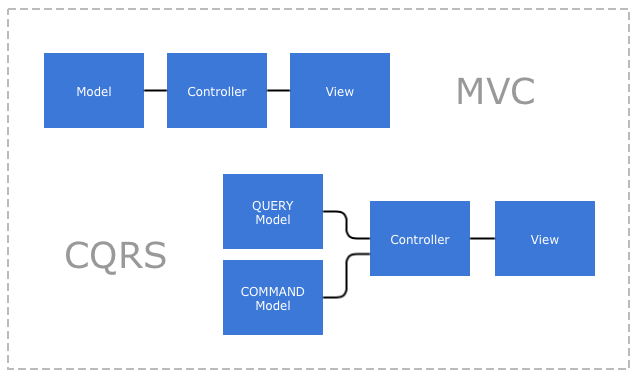
\includegraphics[scale=0.5]{CQRS3}
\end{figure} 


\subsection{How to implement CQRS?}
In complex applications usually happens that different services are integrated and the event's workflow from its birth until its complete execution often goes through different phases(calling different functions, different tasks etc.) while a reading operation just have to query a database to retrieves the needed data. \\
In these cases the ideal solution is to separate the system into two independent models: one for writing operations, which perform changes to the database, and one for reading operations, which do not change anything.
  
\begin{figure} [H]
  \centering
  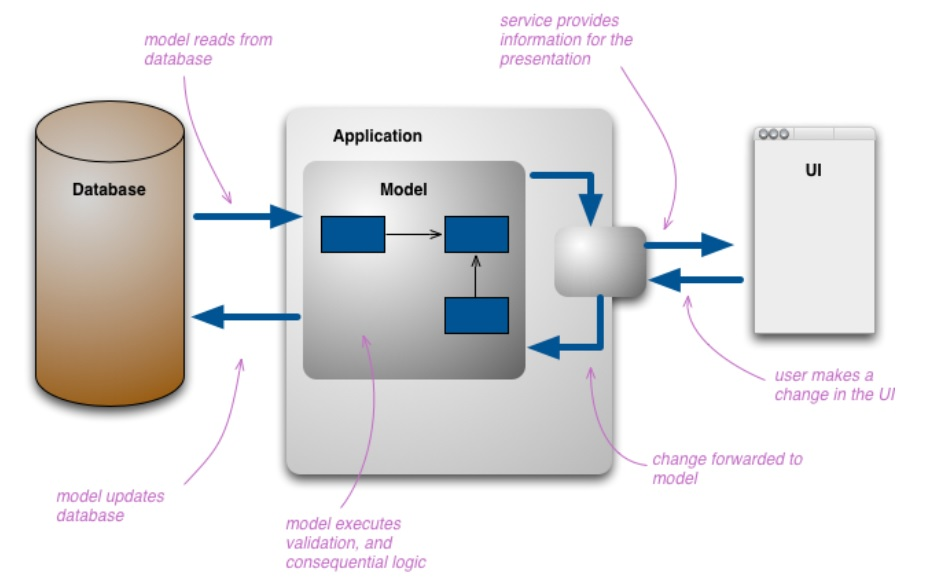
\includegraphics[scale=0.8]{CQRS1} \\
  Example of application model that \textbf{not} adopts CQRS
\end{figure}
\begin{figure} [H]
  \centering
  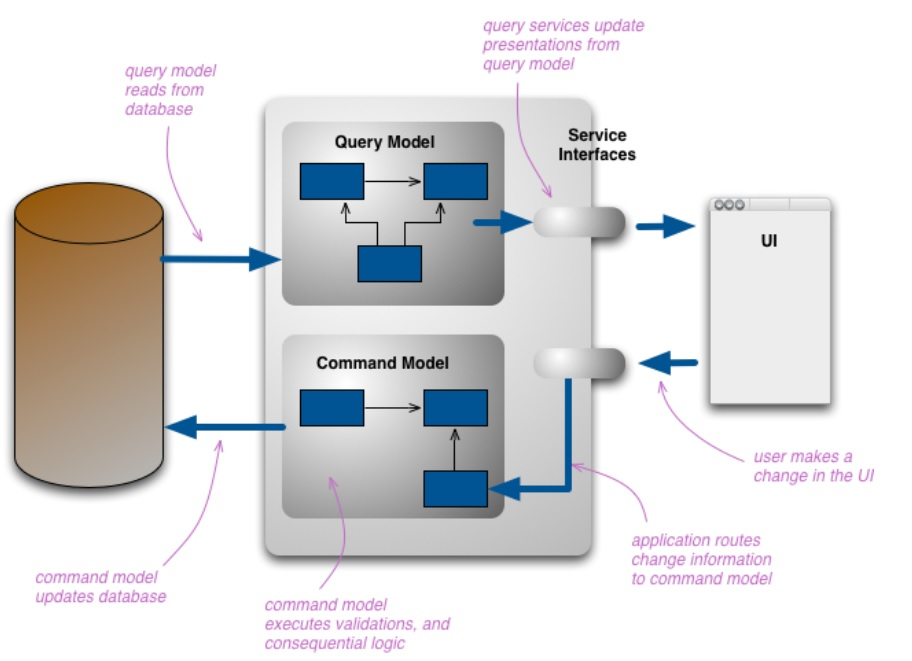
\includegraphics[scale=0.8]{CQRS2} \\
  Example of application model that adopts CQRS \\
\end{figure} 

\section{Event Sourcing} 
\begin{center}
	\emph{"Event Sourcing ensures that all changes to application are stored as a sequence of events."  \\Martin Fowler} \\
\end{center}

\subsection{What is Event Sourcing?}
The core idea of \textbf{Event Sourcing} is that whenever we make a change to the state of a system, we record that state change as an event and we can confidently rebuild the system state by reprocessing the events at any time in the future. It means you do not store the state of an object but all the events impacting its state. Then, to retrieve an object state you have to read the different events related to this object and applied them one by one.
\\
Before storing the event you must validate it because you don't have to store events that generate errors or exceptions.\\ 
When working with an event log can be useful to build snapshots of the working copy so you don't have to process all the events when rebuild the system or every time you need to query the database. For this reason when a new event is stored triggers another function to update the views.

\subsection{When using Event Sourcing?}
Event Sourcing can be used to:
\begin{itemize}
	\item \textbf{Complete Rebuild}: you can completely discard the application state  and rebuild it by re-running the events from the event store on an empty application.
	\item \textbf{Temporal Query}: you can determine the application state at any point in time. This can be used considering multiple time-lines (like branching in a VCS).
	\item \textbf{Event Replay}: if you find that a past event was incorrect, you can replaying from then with the correct event. The same technique can handle events received in the wrong sequence with systems that communicate with asynchronous messaging.
\end{itemize}

\subsection{Event Store}
\textbf{Event Store} is a database's table that contains all the events occurred from the begin.
With event sourcing the event store becomes the principal source of truth and the system state is completely derived from it. \\
Is essential that the table can't be modified and the events that are replayed don't have to be stored again. 
This because the event store can reach huge dimensions and we must avoid to overload it.\\
\begin{figure} [H]
	\centering
	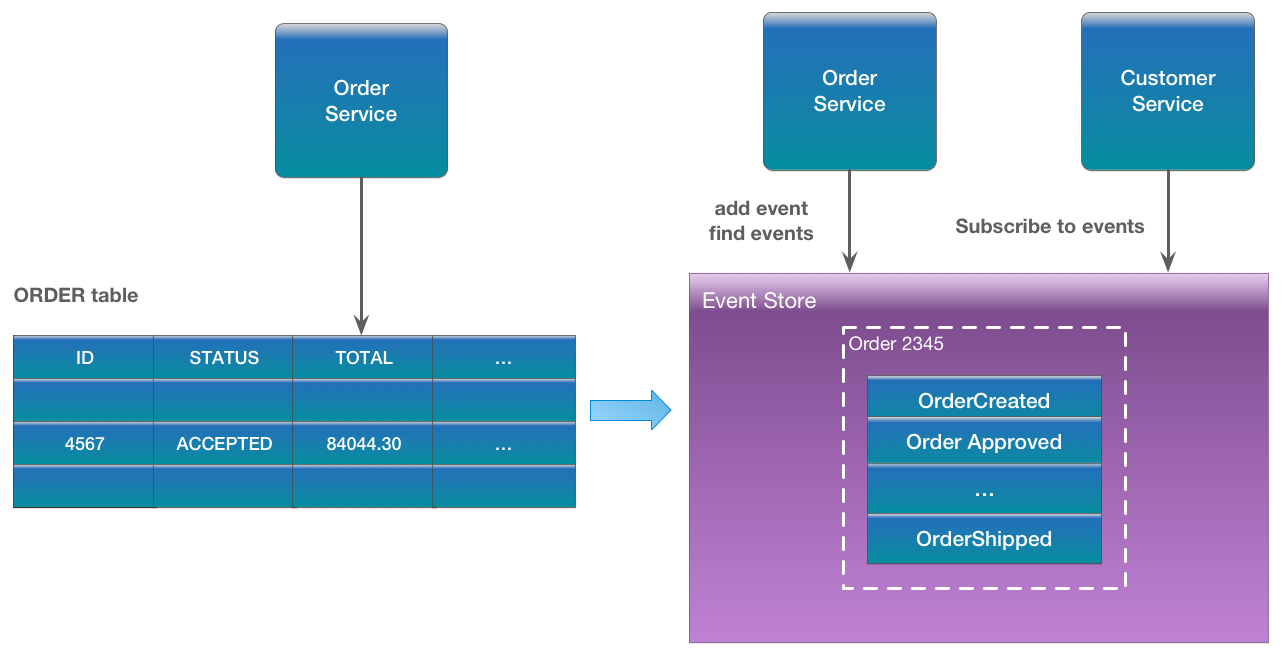
\includegraphics[scale=0.3]{storingevents1} \\
\end{figure}
In a complex system with billions of users the best choice is to implement an event store table for each aggregate object in order to keep track of the events that occurred to a single entity. In this way there are more event stores but this tables have less entries and this increase the speed of a query operation.

\subsection{CQRS and Event Sourcing}
Both patterns are frequently grouped together. Applying Event Sourcing on  CQRS means persisting each event on the write part of our application. Then the read part is derived from the sequence of events. \\
Event Sourcing isn't required when you implement CQRS, but in most of the use cases, CQRS is required when you implement Event Sourcing. This because you have to retrieve a state in \emph{O(1)} without computing \emph{n} different events.

\section{Comparison between cloud providers} 

\subsection{AWS vs Azure vs Google}
Amazon, Microsoft and Google are the three dominant providers in public cloud computing. Each of three has its own set of advantages and your best will depend on your needs. 
\begin{figure} [H]
	\centering
	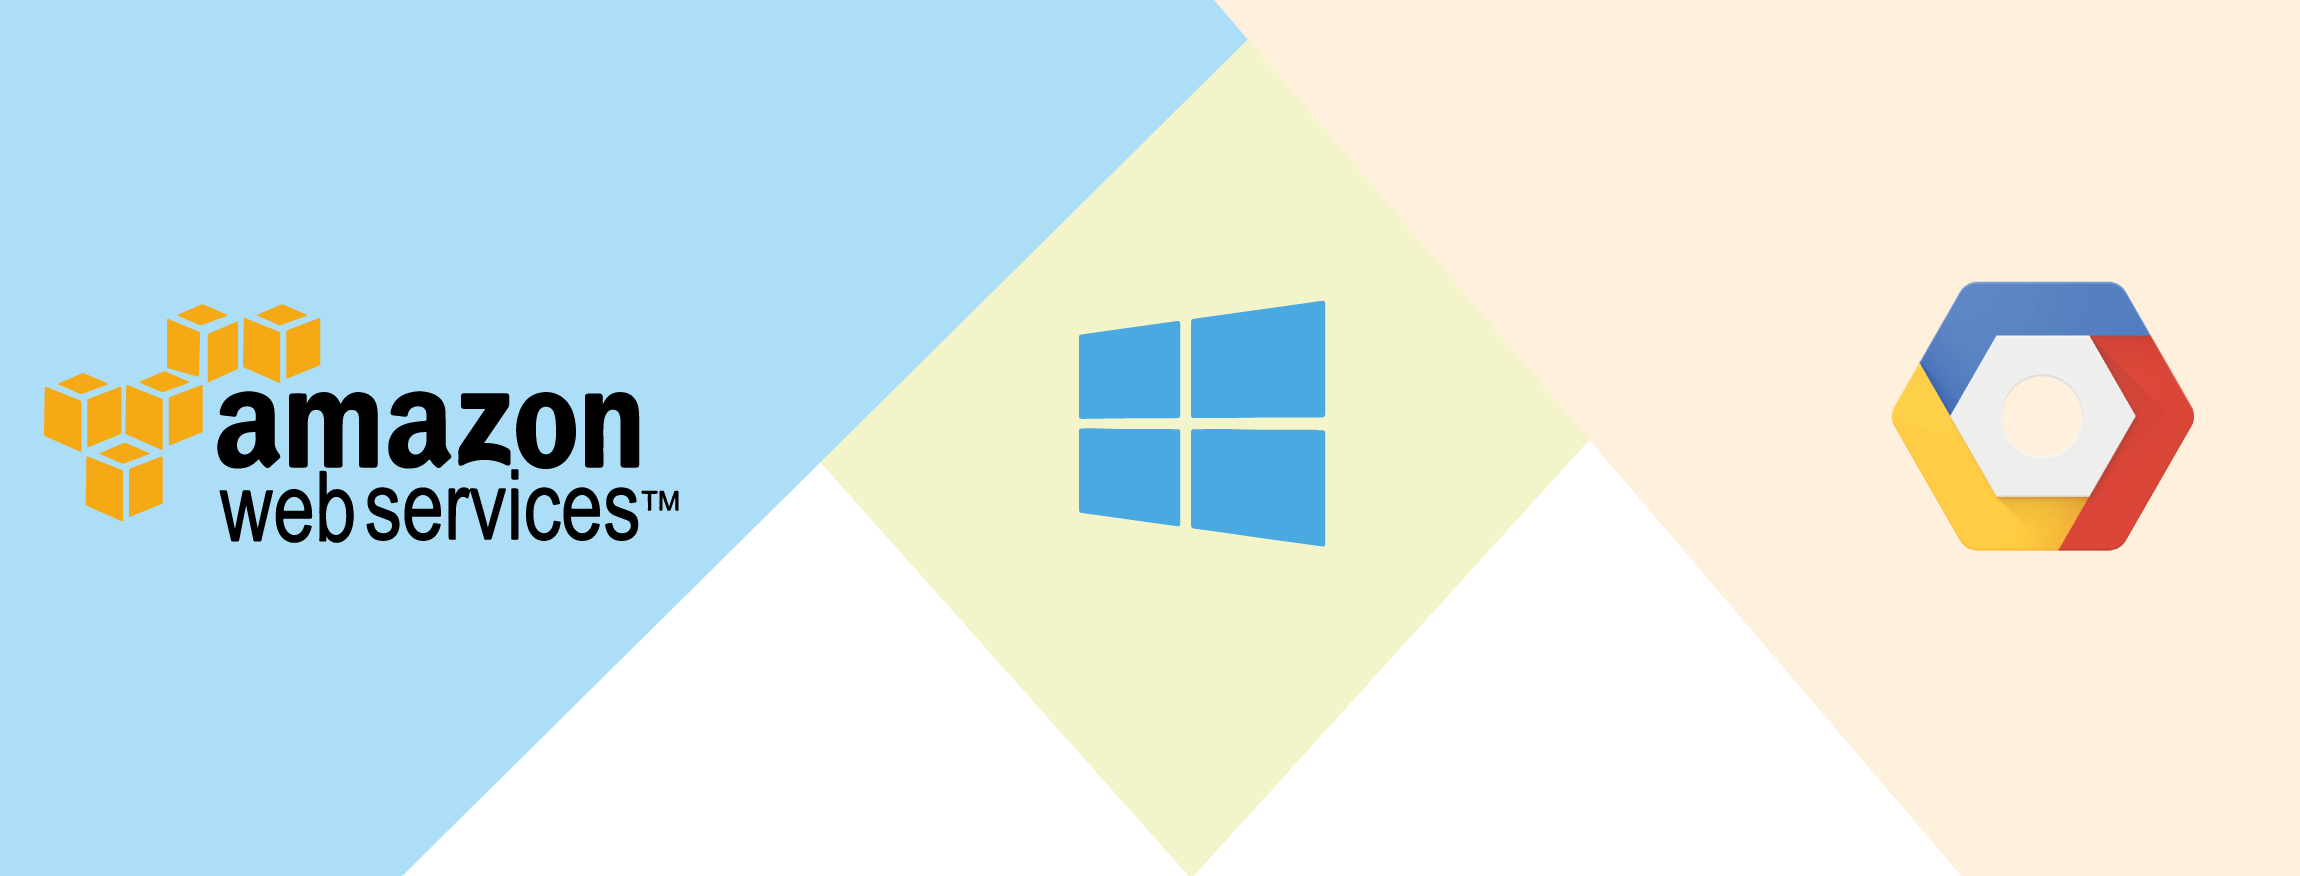
\includegraphics[scale=0.17]{ahp-cloud-providers} \\
\end{figure}

\subsubsection{COMPUTE}
The main compute services are AWS’s Amazon Elastic Compute Cloud (\emph{EC2}), Microsoft Azure’s Virtual Machines and Google Cloud’s Compute Engine. All three boast scalability, top security, flexibility and a wide variety of supported operating systems:
\begin{itemize}
\item \textbf{Amazon}: Elastic Compute Cloud web service provides scalable compute capacity in the cloud. You can easily increase and decrease capacity in minutes and can commission thousands of server instances simultaneously. AWS Auto Scaling monitors your apps and automatically scales capacity to maintain optimal performance at the lowest possible cost;
\item \textbf{Microsoft}: Virtual Machines virtualize a wide range of computing solutions including development and testing, running applications,and datacenter extension. Its open-source software supports a full range of Linux distributions, Windows Server, SQL Server, Oracle, IBM and SAP. Virtual machines can be created for both on-premises servers and on the cloud, and can be integrated to provide global load balancing;
\item \textbf{Google}: Compute Engine creates virtual machines that run in its data centers and worldwide network. It supports instances with up to 160 virtual CPUs, 3.75 TB of memory and persistent SSD and HDD disks up to 64 TB. Google automatically discounts prices for long-running workloads.
\end{itemize}

\subsubsection{STORAGE}
\begin{itemize}
\item \textbf{Amazon}: Simple Storage Service (\emph{S3}) is scalable object storage service. Any amount of data can be stored and protected. Amazon S3 is designed for durability and stores millions of applications from companies all around the world. Its use cases include: backup and restore, disaster recovery, archiving, data lakes and big data analytics, hybrid cloud storage and cloud-native application data;
\item \textbf{Microsoft}: Azure Storage is an all-encompassing data storage service. It includes the following storage types: file, disk, blob, data lake storage and archive; 
\item \textbf{Google}: Cloud Storage is an unified object storage. Google's approach to storage is the most simple and convenient.  It has a single API for all storage classes. Object Lifecycle Management helps you automatically optimize price/performance across classes.
\end{itemize}

\subsubsection{SECURITY}
Amazon, Microsoft and Google are the best when it comes to data security. They all offer expert security guidance and assistance:
\begin{itemize}
\item \textbf{Amazon}: partners offer hundreds of security solutions that complement the existing AWS services. Amazon Inspector automatically assesses your applications for vulnerabilities and deviations from best practices and you may perform penetration testing on your EC2 and RDS instances;
\item \textbf{Microsoft}: Azure Security Center offers a unified view and control of security for all of your on-premises and cloud workloads; 
\item \textbf{Google}: data stored in cloud infrastructure is automatically encrypted and distributed to maximize availability and reliability.
\end{itemize}

\subsubsection{PRICING}
Amazon, Microsoft and Google offer trial versions and free-tier products and services. Each provider offers unique services and special pricing  Also, prices change all the time and it is difficult to get an accurate comparison. \\
Google generally offers the lowest prices, however AWS does offer better deals on some of their long-term commitments. 

\section{Cloud portability}
\subsection{What is cloud portability?}
Cloud \textbf{portability} is the  “\emph{cloud customer’s ability to move applications and data between on-premises and cloud systems, and between cloud services offered by different providers}”. \\
Portability can be broken into two types: \textbf{application portability} and \textbf{data portability}:
\begin{itemize}
\item Cloud application portability is the ability to move an application from one cloud service to another or between a customer's systems and a cloud service. It's important to be able to do that with relative ease;
\item Cloud data portability is the ability to move data among cloud and on-premises systems. This should be done using a mechanism for importing data into the targeted cloud service, typically with an API.
\end{itemize}

\subsection{Cloud portability with containers}
The notion of containerizing applications provides cloud portability. \\
Portability is a key advantage of containers, as developers can easily move a container from a laptop to a test environment and then to production. \\
They take abstraction a layer beyond virtualization. Once an application is running successfully within a container, there is no need to be concern about OS dependencies. Containers are lightweight, portable and consistent across the development, testing and production environments. Containerizing applications reduces the level of effort associated with migration between clouds.

\begin{figure} [H]
	\centering
	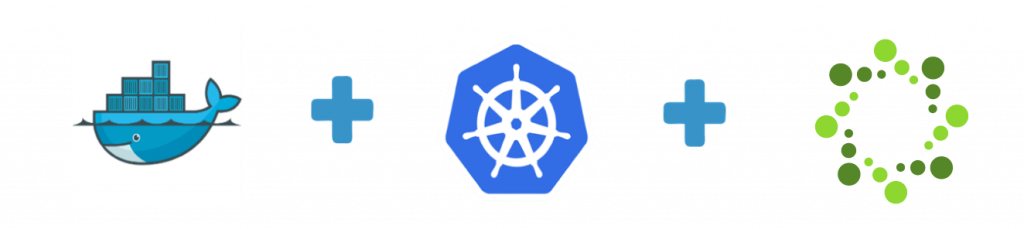
\includegraphics[scale=0.5]{containers} \\
\end{figure}

Thanks to services such as Docker, Kubernetes and OSB API you can achieve application portability in form of containers, the ability to orchestrate the deployment, their scalability and tie services across cloud providers and on-premises to different platforms. The resulting suite maximizes application portability across cloud infrastructure.

\end{document}
